% !TEX root = ../literature.tex
\section{State of the art of interacting with large displays}
We present an overview of research in interaction techniques for cross device interaction, with an emphasis on the natural user interface.\\
By looking at Public Space we found the following topics in HCI: Cross-device Interaction, Large Displays, Multi-device Interaction, Natural User Interface, Proxemics, Social Interaction, Tabletop Interaction, and Tangible Interaction. \\
We used these topics for our inquiry in ACM DigitalLibrary, SpringerLink and Microsoft Research, which matched a total of 56 papers. \\
To narrow down our focus we selected papers that matched a set of strict criteria: (1) The paper should contain one or more interaction techniques, (2) It is important that the techniques are evaluated using either interviews, surveys, field studies or any other research method.\\
The final set contained 34 literature sources which we further examined, by writing a short summary for each paper which included ``title, author's thesis (aim of paper), objectives (goals, summaries), methodologies used, findings, conclusion, and keywords''. 
Using applied thematic analysis different themes were induced on the summaries, which we later categorized into 5 themes: interaction with large displays, interaction with public displays, natural user interactions, cross-device interactions, cross-device natural user interactions.\\
The identified themes and the specific papers correlated to them are presented in Table 1, with full citations in the references section of this paper. 


\begin{table*}[t]
\centering
\begin{tabular}{@{}ll@{}}
\toprule
Theme & Paper \\ \midrule
Interacting with Large displays      &      [1] [3] [32][33] \\
Interacting with Public displays      &       [4] [5] [6] [7] [8] [10] [11] [12] [34] \\
Natural user interactions      &      [9] [13] [14] [15] [16] [17] [18] [19] [30] [31] \\
Cross-device interactions      &      [20] [21] [22] [23] [24] [25] \\
Cross-device natural user interactions      &      [26] [27] [28] [29] \\ \bottomrule
\end{tabular}
\caption{Among the final 34 papers found, we identified 5 themes.}
\label{table:themes}
\end{table*}

% subsections
% !TEX root = ../literature.tex
\subsection{Interacting with Large Displays}
Influenced by Weiser's paper \cite{Weiser:1991} in which he states that ubiquitous computers have to be of different sizes, each suited to a particular task. 
As real power emerges from the interaction of all the different devices, researchers started pushing the boundaries towards constructing large displays used horizontally as tabletop displays or vertically as display-walls.
 
Welnner showed the first examples of a display used as a tabletop -  Digital Desk\cite{Wellner:1993} he utilized optical and acoustic finger detection on the tabletop and also played with the possibility of tactile manipulation of physical objects on the surface. Portfolio Wall was developed at the end of the 90s as a system that utilized a vertical touch-screen display by Buxton\cite{Buxton:2000}. His idea was proposed as a corkboard in digital format used to share work inside the design team.

Rapid progression in the technology for displays and projections, naturally led to lowering of the marginal price, thus ``large displays have moved out of research laboratories into public spaces such as museums, libraries, plazas, and architectural facades, where they present information and enhance experiences'' \cite{Hinrichs:2013:IPD:2478559.2478965}

We can summarize that Public displays is an application of large display therefore examining the latter without the first is a futile action.
% !TEX root = ../literature.tex
\subsection{Interacting with Public Displays}

Rapid progression in the technology for displays and projections, led to considerable proliferation of large displays, thanks also to their capacity to promote activity and social awareness [34], they moved out from research laboratories into public spaces. 
However, ``these displays typically present predetermined feeds offering no interactivity'' [4] states Brignull and Rogers. 
Ten years later Ojala et. al still support this thesis, that ``to date, however, these displays are still used primarily as one-way commercial digital signs.'' [5]. 
Nevertheless researchers continue to combat and change this trend, as such a body of research has formed around interactive public displays. 
A large part of this body presents unique  solutions for installations and devices for particular public settings with specific display technology [6].
Boring and Baur address the problem of crafting interaction techniques that can be used in an array of settings while at the same time maintain some autonomy from the components of public space and different display technology. 
They have done so by developing a ``[...] conceptual framework and technical implementation that rely solely on the public displays and users' mobile devices.'' [7]. By  leveraging cell phone cameras they have enabled from-a-distance interaction with any public-display technology.
From-a-distance interaction using a handheld devices is not the only way to interact with public displays. 
Jacucci et al. adopted touch as a base for their ``Worlds of Information'' system. 
They ``discuss how to design for and evaluate engagement in a public walk-up-and-use installation'' [8]. 
Also, low-cost motion detecting depth cameras permit gesture interactions with displays. 
Gang Ren and his team explain how they used input based on gestures to navigate 3D imagery and how such interaction techniques influence social dynamics around the display. 
They point out that ``for large public displays, gestural interaction can enhance the experience of not only the current user but also the people sharing that public space or activity.'' [10].
This observation led to value which could be exploited, as Lucero et. al. tried to do. 
Focusing on the collaborative and cross-device side, Lucero et. al. created MobiComics with the purpose to ``explore shared collocated interaction with mobile phones and public displays in indoor public place.'' [11]. 
Valkanova et. al tried to focus on the discussion and natural user interaction side by creating MyPossition, a ``public display in the form of a large projection, featuring an interactive poll visualisation.'' [12] which aimed to aggregate public opinions for local issues by utilizing voting with gestures.
In this section we explored literature on interacting with public displays. 
By doing so, two clusters of research papers were formed, one on cross-device interaction, and another on natural user interaction, which defines the need for their further examination in relation to the main topic.
% !TEX root = ../literature.tex
\subsection{Natural User interaction}
Natural user interactions are underlaying for the natural user interface. The "natural" in Natural User Interface is about how users feel and what they do when using a product. A product should take full advantage of the user's capabilities; the trick lies in making the user feel that it is natural from the start and not after a long time practicing. That does not mean that the product should be designed towards no learning requirements; it can be a better solution to make the user learn how to deal with the technology than making the technology deal with the complexity of humans. An example would be Apple's Newton Message Pad which was promised to understand human handwriting. The results were bad as the handwriting recognition was insufficiently robust. The successor Palm Pilot(1997) by Palm computing had more success, as the creators recognized the limitations of their technology. They developed an input language similar to roman characters that the users had to learn, however the experience felt natural because the recognizer worked so well \cite{Wigdor:2011}.

In 2001 Keefe et al. \cite{Keefe:2001} created a 3D virtual reality painting system where they used tangible items like a brush and cups for selecting brush type, to create an intuitive interface for artists who might not be familiar with virtual reality. The brush is tracked in the 3D space and the color palette is opened by making a circular gesture while holding the brush in an upward position; a color selection is made by moving the brush to a color and tilting the brush into another direction.
For advanced users a tracked glove can be used on the non-dominant hand to provide quick access to changing color and brush size.
The tracking however requires special cabled equipment, which results in additional weight on the hands and reduces the free movement. 

Microsoft released the Kinect for Xbox 360 in 2010\cite{KinectFiction:2010} and the Kinect for Windows in 2012\cite{KinnectPower:2012}. The Kinect has a depth sensor, color camera sensor, and four-element microphone array. We found that the Kinect has been a tool for much research, many of them utilizing the depth sensor, which is the case of the following papers:\cite{Wilson:2010, Aigner:2012, Walter:2014}.

Wilson \cite{Wilson:2010} wanted to explore the application of depth-sensing cameras to detect touch on a tabletop. He found it to be less precise than touch screens, but with three advantages. The surface does not need to be instrumented; The surface is not required to be flat; and the information about the shape of the users and their arms can be exploited in useful ways, such as determining hover state or whether multiple touches is from the same user \cite{Wilson:2010}.

Motivated by surface and tabletop systems expansion to include proximity sensing, Aigner et al.\cite{Aigner:2012} looks at the Point-and-Click interface and User-Defined Interface(UDI). They find that Vogel and Balakrishnan \cite{Vogel:2005} built a Point-and-Click interface for large screen displays which simulates mouse input, and that several issues was discovered: precision in pointing, ambiguity of finger movements, and lack of physical feedback. They describe that it has been common to elicit gestures by applying the UDI methodology, but researchers have found that there is little consensus among users in association between gestures and their expected effect.

Aigner et al.\cite{Aigner:2012} believe that gesture languages have to be designed rather than observed, however a key limitation is the lack of guidelines for designing such languages.
They developed a Gesture type classification scheme based on the taxonomy of Karam and Schraefel \cite{Karam:2005} .
From their experiment they found that the participants used  a  wide  variety  of  gestures  to accomplish  the  same  effect, but the  type  of  gesture was  often  consistent  across  time and participant. Hence, their results suggest that \emph{"classifying by type reveals a much greater degree of consistency"} compared to eliciting gestures by using the UDI methodology. 

Walter et al.\cite{Walter:2014} state that today's public displays only show predefined contents that passers-by are not able to change and argue that displays would benefit from techniques for interacting with large displays. They propose a design space for hand-gesture based mid-air selection techniques based on analysis of differences and similarities of existing mid-air selection techniques in NUI frameworks, commercial products and related work. From two lab studies they derived 4 selection techniques that supports immediate usability. In a field study they found that the 4 techniques performed equally and conclude that designers can choose freely between those 4 techniques.
They give their recommendation for designing of interactive public displays, that allows users to select options using mid-air gestures; and believe that their findings will make the platform of interactive public display more attractive to users.

In this section we have explored literature on NUI, showing some of the early development and some of the later development where the Kinect has been used. From this we can deduce that there have been a focus on exploring the application of depth-sensing cameras as well as understanding and designing mid-air hand gestures.
Using the Kinect as a tool we can achieve interaction in a limited 3D space without the need for additional tools, such as tracked controllers or gloves. The Kinect can be used to achieve touch detection on non-instrumented surfaces or in midair by using the depth sensor to detect distance and recognize gestures.  Aigner et al.'s and Walter et al.'s results have been recommendations and guidelines for selecting and designing hand gestures for interacting with the Kinect. Aigner  et al.\cite{Aigner:2012} believes that a gesture language has to be designed instead of observed. Through the observation of participants communicating by using gestures in a lab study, they discover that the participants often used the same type of gesture to achieve a desired effect.
Walter et al. argues that public displays would benefit from techniques for interacting with large displays. They made a designspace which they tested to derive the selection techniques that supports immediate usability. In a field study they found that their 4 derived selection techniques performed equally and concludes that designers can choose freely among them. With these findings we are now aware of several applications where the Kinect can be used for interaction and which types of interaction techniques that provides the user with a good experience when using the Kinect.
% !TEX root = ../literature.tex
\subsection{Cross-Device Interaction}
Interaction was understood, usually, as single user using a single device, this was almost always a desktop computer\cite{Levin:2014}. We have moved from this protocol into the more complex world of cross device interaction, as such it is important to give definition of this phenomenon.\\

\emph{"Cross-device interaction is the type of interaction, where human users interact with multiple separate input and output devices, where input devices will be used to manipulate content on output devices within a perceived interaction space with immediate and explicit feedback."} \cite{Scharf:2013}.\\

Rikimoto presents an early envisionment of this idea. In his work the technique he proposed was a Prick-and-Drop technique, he explains that "Pick-and-Drop allows a user to pick up an object on a display and drop it on another display as if he/she were manipulating a physical object." \cite{Rekimoto:1997}. The author discusses how, even though from a functional point of view, the technique does not differ from a traditional remote copy command, the added extra layer of physicalness makes a difference for the user. \emph{"understanding that we are living in a fusion of physical (real) and virtual (computer) worlds. Each has its own advantages and disadvantages. Pick-and-Drop, for example, adds physicalness to user interfaces, because we feel that traditional data transfer methods are too virtual and hard to learn due to their lack of physical aspects"} \cite{Rekimoto:1997} remarks the writer.\\
Perhaps one of the earliest working systems illustrating CDI is by Myers et al.
\cite{Myers:2001} one of the application realized within their \emph{Pebbles project} is SlideShow Commanded that utilized Personal Devices Assistants (PDA) to control a PowerPoint presentation running on other computer or laptop.
It was possible not just moving between slides, but also scribbling and writing on the PDA slides, while annotations are shown on the presentation for the audience.\\

Hamilton and Wigdor have a more modern reading on this, they wanted to see how the users would utilize a group of tablets with cross-device capabilities. For this task they crafted\emph{ "Conductor, a prototype system that combines a set of interaction techniques designed to enable single user, cross-device applications, manage cross-device relationships, and enable easy functionality chaining."} \cite{Hamilton:2014}.\\

Radle et. al continued with the multi-tablet cross-device interaction, however their focus shift to the competing interaction techniques. They define three categories: \begin{enumerate}
	\item Synchronous gestures
	\item Spatially-agnostic interactions
	\item Spatially-aware interactions. 
\end{enumerate} They found \emph{"the results indicate that spatially-aware techniques are preferred by users and can decrease mental demand, effort, and frustration, but only when they are designed with great care."} \cite{Radle:2015}.\\

Cross interaction between the same type of device are not the only one. Schmidt et al. propose a cross-device interaction style for mobiles and surfaces. The researchers point out that \emph{"natural forms of interaction have evolved for personal devices that we carry with us (mobiles) as well as for shared interactive displays around us (surfaces) but interaction across the two remains cumbersome in practice"} \cite{Schmidt:2012}; so in order to overcome this they propose to use mobiles as tangible input on the surface in a stylus like fashion.\\

Boring et. al. takes cross-device interaction with mobiles and large displays. Their idea is to combine the largescale visual output and the mobile phone as an input, to enable a channel of communication which is bidirectional with the large public display. To do this they \emph{"propose and compare three different interaction techniques (Scroll, Tilt and Move) for continuous control of a pointer located on a remote display using a mobile phone"} \cite{Boring:2009}.\\
Skov et al. \cite{Skov:2015} illustrate six different cross-device interaction techniques for the case of card playing in \emph{Investigating Cross-Device Interaction techniques}.
A player can see their own cards on their phone and use three different techniques for playing a card from the handheld to the tablet, which is placed on a table.
In the other direction, i.e. when drawing a card, the player also has three techniques to choose from.
The usability study aims to quantitatively evaluate each of the techniques and showed that there is a difference in time and number of errors between the techniques. \\

The current paragraph exemplifies that designing a solution for cross-device interaction can be complex, as such to understand  unique properties and challenges of the domain is a must. The early literature focuses on interaction support. Gradually this evolves to understanding the interaction process itself in different device environment i.e. large display and hand-held device, and multiple hand-held device.With the body of knowledge on cross-device, and natural interactions as part of large display, a logical step is to look and ask if researchers have tried to combine CDI and NUI in public spaces with large displays.

% !TEX root = ../literature.tex
\subsection{Cross-Device Interaction Natural User Interface}
Infusing the two fields could offer new concepts and potential ideas, as such an inquiry of the current literature would be beneficial. 
An illustrative example, on transitioning from one to another area, would be Greenberg et al. work \cite{Greenberg:2011} who expand on a concept from Psychology, which states that different distance between people can explain their relation, by adapting it for use in HCI, they do so by concerning distance, not only between people, but between all objects such as people, electronic devices and analogue objects. Their main contribution is in defining five proxemic dimensions: \emph{Distance, Orientation, Movement, Identity} and \emph{Location}. This dimensions can be used to help devices, in a system ecology , to recognize their current context, distance to other people or devices, and can help creating interconnectivity between entities. 

Marquardt work, that proposes to use spatial information - proxemics {\em``[...] to mediate people's interactions with digital devices, such as large digital surfaces or portable personal devices.''} \cite{Marquardt:2011}, gives an illustration of the use within cross-device. He presents design of development tools for programmers creating proxemic-aware systems, his aim is {\em``to create techniques that allow people to seamlessly and naturally connect to and interact with the increasing number of digital devices.''} \cite{Marquardt:2011}. 


Marquardt et. al. later expand this idea by increasing the number of dimensions i.e. he augments proxemic principles with theories of F-formation and micro-mobility, his creation is a system that uses combination of Kinect sensors and accelerometer data, which was combined to determine the locations and orientation of users in an instrumented environment . This information was used to facilitate a number of real-time interactions between user devices, as the author writes {\em``[...]a system that explores cross-device interaction using two sociological constructs. First, F-formations concern the distance and relative body orientation among multiple users, which indicate when and how people position themselves as a group. Second, micro-mobility describes how people orient and tilt devices towards one another to promote fine-grained sharing during co-present collaboration.''} \cite{Marquardt:2012}. Combining these two aspects, new techniques of cross-device interaction with emphasis on fluid and smooth communication can be designed argues the author. For instance, tilting a device by a small angle may trigger an information sharing process with other devices within proximity\\ 


Proxemics is one of the ways to create cross-device natural user interaction.
Bragdon et al. propose using a system that combines touch + air gesture hybrid interactions.
They aim to design, implement and test a system that allows a group of users to interact using air gestures and touch gestures. 
The purpose is to increase control, support democratic access, and share items across multiple personal devices such as smartphones and laptops where the {\em``primary design goal is fluid, democratic sharing of content on a common display.''} \cite{Bragton:2011}. This method enables access, control and sharing of information through several different devices such as multi-touch screen, mobile touch devices, and Microsoft Kinect sensors. In a formative study, professional developers were positive about the interaction design, and most felt that pointing with hands or devices and forming hand postures are socially acceptable. 
% !TEX root = ../literature.tex
\subsection{Summary}
Many researchers spend time and effort to explore how large displays can improve people's experiences. 
With the shift from private to public settings the explored solutions changed. 
It was highly impractical to put wires on people who wanted to use an installation naturally in a public environment [9].
With this limitation came different approaches for solving it. 
We identified two different areas which deals with it, we present them in \Cref{fig:litreview}.

\begin{figure*}
\centering
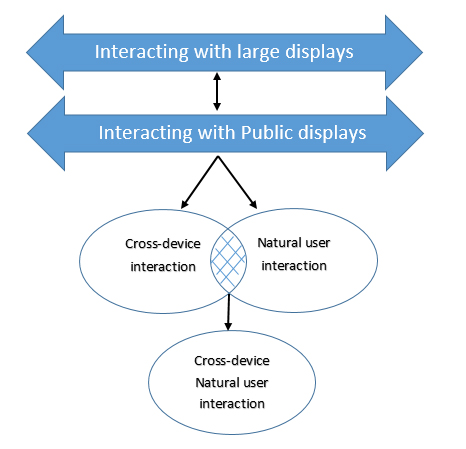
\epsfig{file=images/litreview-fig1.jpg, width=0.5\textwidth}
\caption{\todo{Write caption}}
\label{fig:litreview}
\end{figure*}
 
The fields of natural user interactions and cross-device interactions were thoroughly examined. 
We were surprised to see that research in combining features from the two areas is slim even though they are complementary to each other. 
There was research that was done [26, 27, 28, 29]. 
Interaction-techniques were evaluated with 3-6 people using qualitative surveys in [27,28,29] and without qualitative surveys in [26].

In summary, we can see research opportunities in further exploration of cross-device natural user interactions technique for large displays. 
Firstly, as handheld devices become thinner and lighter and spatially-aware technologies, such as Kinect, continue to evolve, this opens a potentially rich space of aforementioned techniques. 
Secondly, we see opportunities in quantitative aspect, for example comparative study of different interaction techniques. 
